\documentclass{beamer}
\setbeamertemplate{subsection in toc}[sections numbered]
\setbeamersize{text margin left=7mm,text margin right=7mm}

%
% Choose how your presentation looks.
%
% For more themes, color themes and font themes, see:
% http://deic.uab.es/~iblanes/beamer_gallery/index_by_theme.html
%
\mode<presentation>
{
  \usetheme{default}      % or try Darmstadt, Madrid, Warsaw, ...
  \usecolortheme{beaver} % or try albatross, beaver, crane, ...
  \usefonttheme{default}  % or try serif, structurebold, ...
  \setbeamertemplate{navigation symbols}{}
  \setbeamertemplate{caption}[numbered]
  %\setbeamertemplate{footline}[frame number]
} 
\usepackage{xcolor}
\newtheorem{proposition}{Proposition}[section]
\usepackage[english]{babel}
\usepackage[utf8]{inputenc}
\usepackage{amsmath,amssymb,tikz-cd}
\usetikzlibrary{positioning}
\tikzset{main node/.style={circle,fill=black,draw,minimum size=.25cm,inner sep=0pt},
            }
\usepackage[upright]{fourier}
\usetikzlibrary{babel}
\usepackage[backend=bibtex,style=numeric-comp,natbib=true]{biblatex}
\addbibresource{references.bib} 
\usepackage[autostyle=true]{csquotes}
\usepackage{graphicx,multicol,caption}
\title[Your Short Title]{Volume of simplicial complex polytopes}
\author{Eliana Tolosa and Jerónimo Valencia}
\institute{San Francisco State University and Universidad de los Andes}
\date{December 17, 2020}

\begin{document}

\begin{frame}
  \titlepage
\end{frame}


\begin{frame}{Motivation}
    Why do we care about calculating volumes?
    \begin{itemize}
    \item It is a hard to compute volumes of polytopes: It is a $\#P$-hard to compute the volume of a $d$-dimensional polytope $P$ presented by its facets.
    \pause
    \vspace{0.5cm}
    \item It is related to other problems in mathematics:
    \pause
        \begin{itemize}
            \item (Algebraic Geometry) If $P$ is an integral polytope, the normalized volume of $P$ is the degree of the toric variety associated to $P$.
            \pause
            \item (Computational Algebraic Geometry) Given $f_1,\dots, f_n$ generic polynomials in $\mathbb{C}[x_1,\dots,x_n]$, the number of isolated solutions of $f_1=0, \dots, f_n=0$ is $$n! \text{Vol}(New(f_1), \dots, New(f_n)).$$
            \pause
            \item (Combinatorics) Volumes count things. (Eulerian numbers, Catalan numbers, binomial coefficients, trees, reverse parking functions, $\dots$)
        \end{itemize}
    \end{itemize}
\end{frame}


\begin{frame}{Motivation}
\begin{theorem}
The volume of the regular permutahedron $P_n(n,n-1,\dots, 2,1)$ is the number of trees on $n$ labelled vertices, this is $n^{n-2}$.
\vspace{0.6cm}
\end{theorem}
\begin{center}
    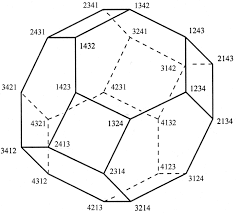
\includegraphics[scale=0.5]{images/Unknown.png}
\end{center}

\end{frame}


\begin{frame}{Motivation}
\begin{theorem}[Postnikov-2005]
There is a formula to calculate the volume of the \textbf{generalized permutahedron} which involves a sum over all G-\textit{draconian sequences} $(a_1, \dots, a_m)$.
\end{theorem}

\end{frame}



\begin{frame}{Understanding the Theorem}
    A \textbf{generalized permutahedron} $P_z^n(\{z_I\})$ is a polytope obtained from a regular permutahedron by a parallel traslation of its faces.
    
    Its $H$-representation is:
    $$P_z^n(\{z_I\}) = \left\{ \Vec{x}\in\mathbb{R}^n \, \mid \, \sum_{i\in[n]}x_i = z_{[n]} \text{ , } \sum_{i\in I}x_i \geq z_I \text{ for proper subsets }I\subset [n]\right\}$$
    where $\{z_I\}_{I\subset [n]}$ is a set of numbers such that $z_I + z_J \leq z_{I\cup J} + z_{I \cap J}$.

\end{frame}

\begin{frame}{Generalized Permutahedra}
 For any $I\subseteq [n]$ fix a non-negative real number $y_I$. 
 Define the polytope $$P_y^n(\{y_I\}) = \sum_{I\subseteq [n]}y_I\Delta_I.$$
 \begin{proposition}
 Let $\{ y_I\}$ a collection of non-negative real numbers indexed by $I \subseteq [n]$ and define the numbers $\{z_I\}$ by $z_I = \sum_{J\subseteq I}y_J$. Then,
 $$P_z^n(\{z_I\}) = P_y^n(\{y_I\}).$$
 \end{proposition}
 
Then we can represent generalized permutahedra as weighted Minkowski sums of the coordinate simplices, that is
$$\sum y_I\Delta_I$$.
\end{frame}

\begin{frame}{Generalized Permutahedra}
 The class of generalized permutahedra includes interesting families of polytopes such as associahedra, cyclohedra, graph associahedra, Pitman-Stanley polytopes, graphical zonotopes among others.
 \begin{center}
      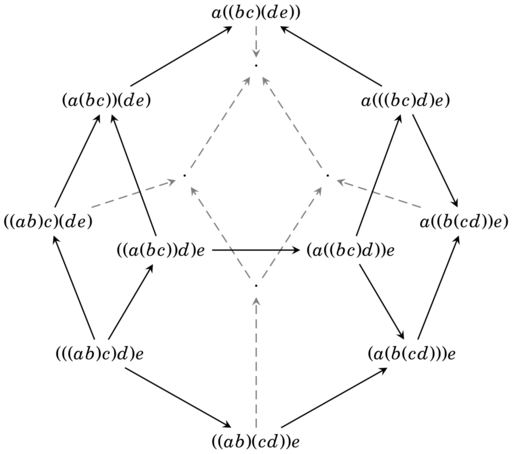
\includegraphics[scale=0.25]{images/Associahedron_K5_front_512.png}
      \hspace{1cm}
      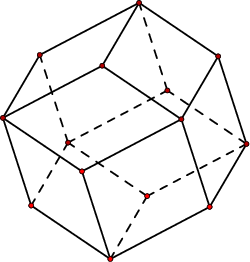
\includegraphics[scale=0.22]{images/7-Figure2-1.png}
      \includegraphics[scale=0.35]{images/Captura de Pantalla 2020-12-16 a la(s) 7.46.15 p. m..png}

 \end{center}

\end{frame}

\begin{frame}{Draconian sequence}
\begin{definition}[Dragon Marriage Condition]
Imagine that in a medieval town there are $n$ brides, $n-1$ grooms and a dragon. We know all the possible pairs of brides and grooms that do not mind to marry each other. One day, the dragon comes to the town and takes one of the brides. When is it possible to match the remaining brides and grooms no matter what the choice of the dragon was?
\end{definition}

\end{frame}

\begin{frame}{Example DMC}
    \begin{center}
    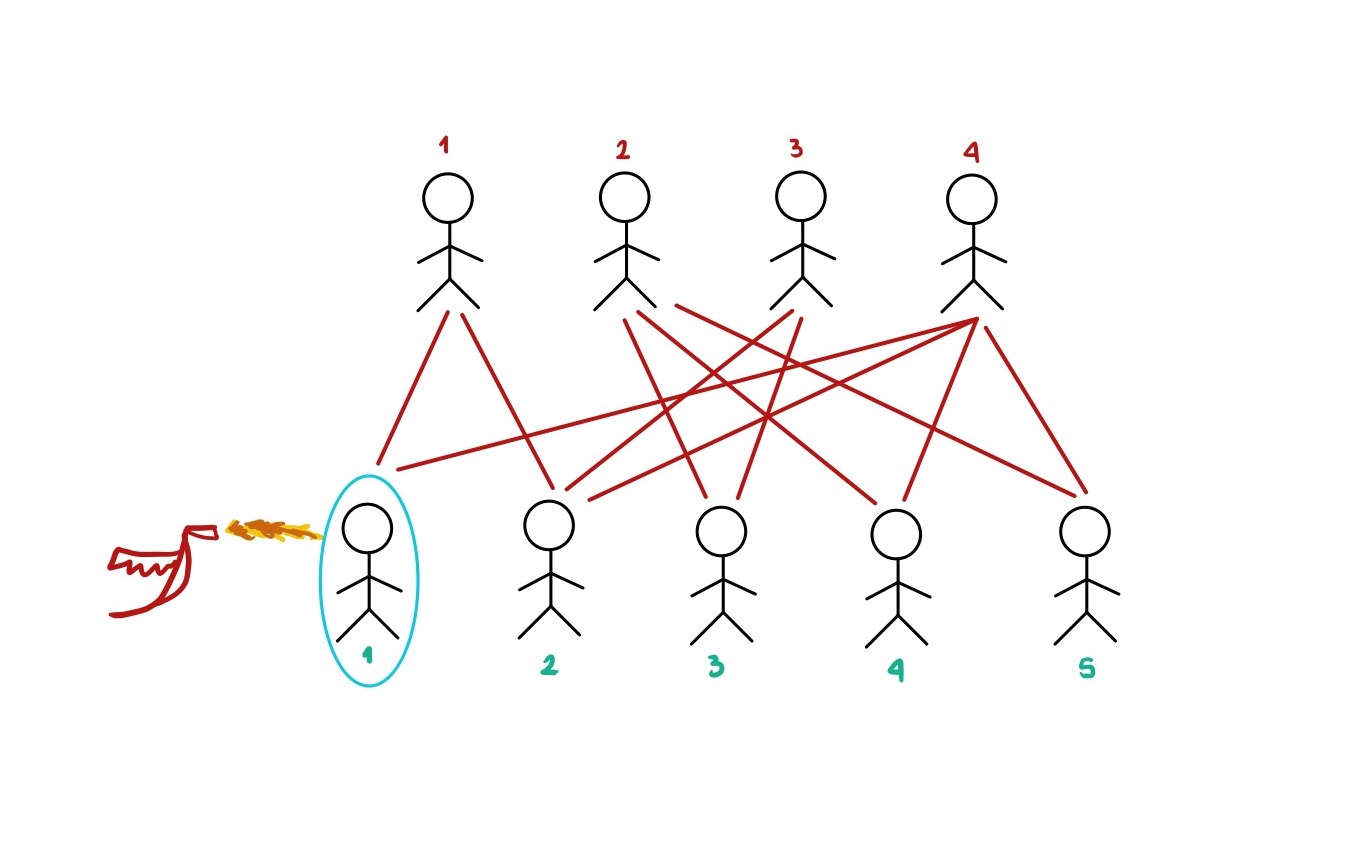
\includegraphics[scale=0.18]{images/DragonMarriageCondition.jpeg}
\end{center}
In this case $I_{\color{red}1}= \{\color{green}1 \color{black},\color{green}2\color{black}\}$, $I_{\color{red}2}= \{\color{green}3\color{black},\color{green}4\color{black}, \color{green}5\color{black}\}$, $I_{\color{red}3}= \{\color{green}2\color{black},\color{green}3\color{black}\}$, $I_{\color{red}4}= \{\color{green}1\color{black},\color{green}2\color{black}, \color{green}4\color{black},\color{green}5\color{black}\}$.
\end{frame}

\begin{frame}{Draconian Sequence}
\begin{definition}[Draconian Sequence]
 Using the notation $I^{(a)}$ for the subset $I$ repeated $a$ times, a sequence of non-negative integers $(a_1, a_2, \dots, a_m)$ is a G-\textit{draconian sequence} if the sequence of subsets $I_1^{(a_1)}, \dots, I_m^{(a_m)}$ satisfies the dragon marriage condition.
\end{definition}
\end{frame}

\begin{frame}{Motivation}
\begin{theorem}[Postnikov-2005]
The volume of the \textbf{generalized permutahedron} $P_G(y_1, \dots, y_m)$ is
$$\text{Vol} \left (P_G(y_1,\dots,y_m)\right )= \sum_{(a_1,\dots, a_m)} \frac{y_1^{a_1}}{a_1!}\dots \frac{y_m^{a_m}}{a_m!},$$
where the sum is over all G-\textit{draconian sequences} $(a_1, \dots, a_m)$.
\end{theorem}
\end{frame}


\begin{frame}{Sketch of the proof}

    \begin{enumerate}
        \item Writing the generalized permutahedron $P_G(y_1,\dots,y_m)$ as a \textit{Minkowsky sum} of simplices $\Delta_{I_{i_1}}, \dots, \Delta_{I_{i_{n-1}}}$ we obtain,
        $$\text{Vol}P_G(y_1, \dots, y_m)= \sum_{i_1,\dots, i_{n-1}}\text{Vol}(\Delta_{I_{i_1}}, \dots, \Delta_{I_{i_{n-1}}})y_{i_1}\cdots y_{i_{n-1}},$$
where the sum is over all $i_1,\dots, i_{n-1} \in [m]$.
\pause
\vspace{0.5cm}
       \item Claim:
       $$\text{Vol}(\Delta_{J_1}, \dots, \Delta_{J_{n-1}})=
  \begin{cases}
    \frac{1}{(n-1)!} \quad \text{if } J_1, \dots, J_{n-1} \text{ satisfy the DMC}\\
0 \quad \text{otherwise.}
\end{cases}  $$

    \end{enumerate}

\end{frame}

\begin{frame}{Sketch of the proof}
\begin{enumerate}
\setcounter{enumi}{2}
    \item Consider the system of equations

\begin{center}
    $$\begin{cases}
      \sum_{j\in J_1} \beta_{1,j}t_j=0,\\
      \quad \vdots\\
      \sum_{j\in J_{n-1}} \beta_{n-1,j}t_j=0.
    \end{cases}$$
\end{center}

\pause
\vspace{0.5cm}
\item Using \textit{Bernstein's Theorem}, this system has exactly
$$(n-1)! \text{Vol}(\Delta_{J_1}, \dots, \Delta_{J_{n-1}})$$ isolated solutions in $(\mathbb{C}\backslash \{0\})^{n-1}$ for generic coefficients $\beta_{i,j}\in \mathbb{C}$ for $j \in J_i$.
\end{enumerate}
\end{frame}

\begin{frame}{Sketch of the proof}
\begin{enumerate}
\setcounter{enumi}{4}
    \item Using \textit{Cramer's rule} we can find that the system has a single isolated solution in $(\mathbb{C}\backslash\{0\})^{n-1}$ if and only if all the maximal minors of $B$ are nonzero. Where $B$ is the matrix of the coefficients of the system of equations. If this does not happen, there are not isolated solutions.
    \pause
\vspace{0.7cm}
    \item The condition on $B$ of having nonzero maximal minors is equivalent to the \textit{Dragon Marriage Condition}.
    
\end{enumerate}
\end{frame}

\begin{frame}{But...}
    We have a formula for calculating the volume of generalized permutahedra,
    \textbf{but} finding the $G$-draconian sequences is a high complexity problem. \\
    
    \pause
    \vspace{0.5cm}
    We should then restrict or family of polytopes to:
    \begin{itemize}
        \item Try to give a nicer interpretation of the $G$-draconian sequences.
        \item Try to find a nicer formula for the volume of this restricted family
    \end{itemize}
    \vspace{0.5cm}
    \pause
    We will focus on the family of \textbf{simplicial complex polytopes}.
\end{frame}

\begin{frame}{Simplicial complex polytopes}
    \begin{definition}
        Given a simplicial complex $C$, we define the \textbf{simplicial complex polytope} $P_C$ as the Minkowski sum of the simplices comprising the complex. That is, if $C = \{ I_1,\ldots,I_n\}$ then $P_C = \sum_{i=1}^n \Delta_{I_i}$ where $\Delta_I := \text{conv}\{ \Vec{e}_i \, \mid \, i\in I \}$. 
    \end{definition}

\begin{columns}
\hspace{0.5cm}
\begin{column}{0.2\textwidth}
    
    \begin{center}
     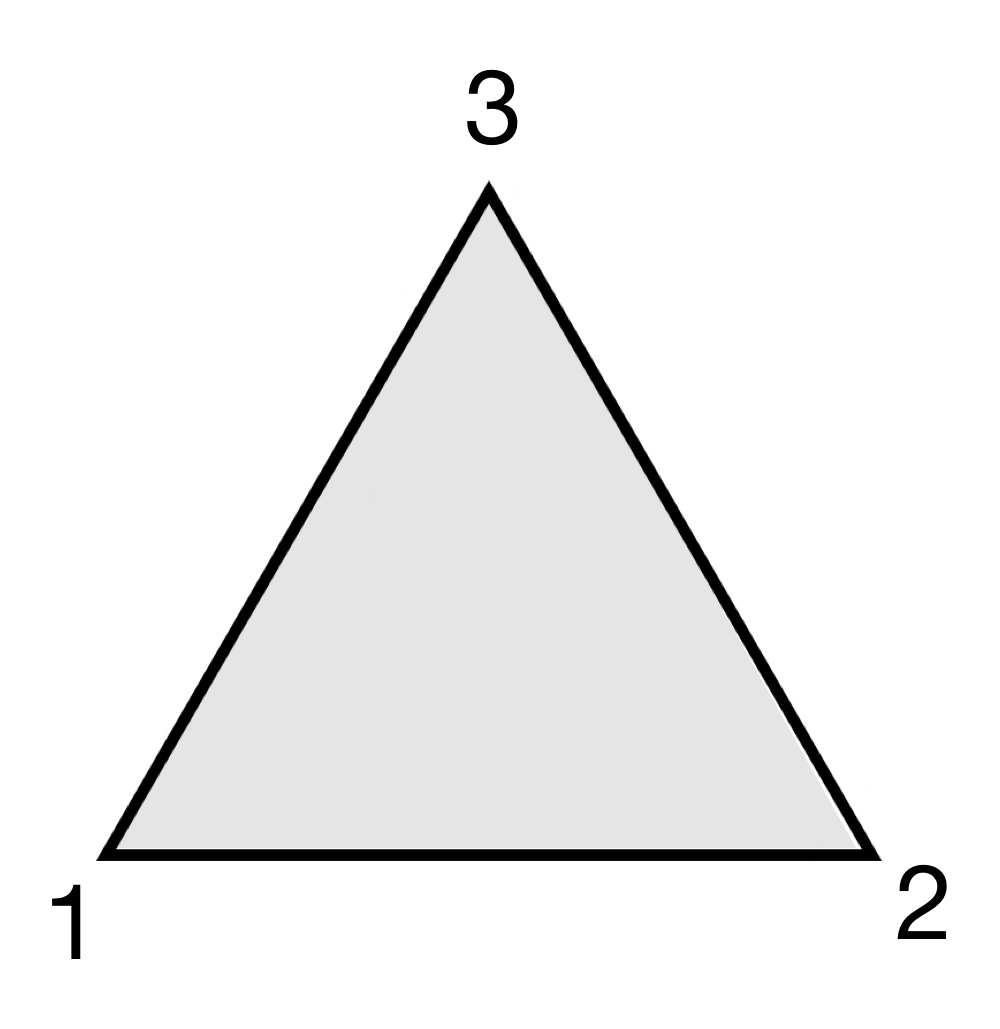
\includegraphics[scale=0.06]{images/C_3.png}
     \end{center}
\end{column}
\begin{column}{0.1\textwidth}                $$\longrightarrow$$
\end{column}
\begin{column}{0.3\textwidth}
    $$\Delta_{12}+\Delta_{13}+\Delta_{23}+\Delta_{123}$$
\end{column}
\begin{column}{0.1\textwidth}
   $$\longrightarrow$$
\end{column}
\begin{column}{0.3\textwidth}  %%<--- here
    \begin{center}
     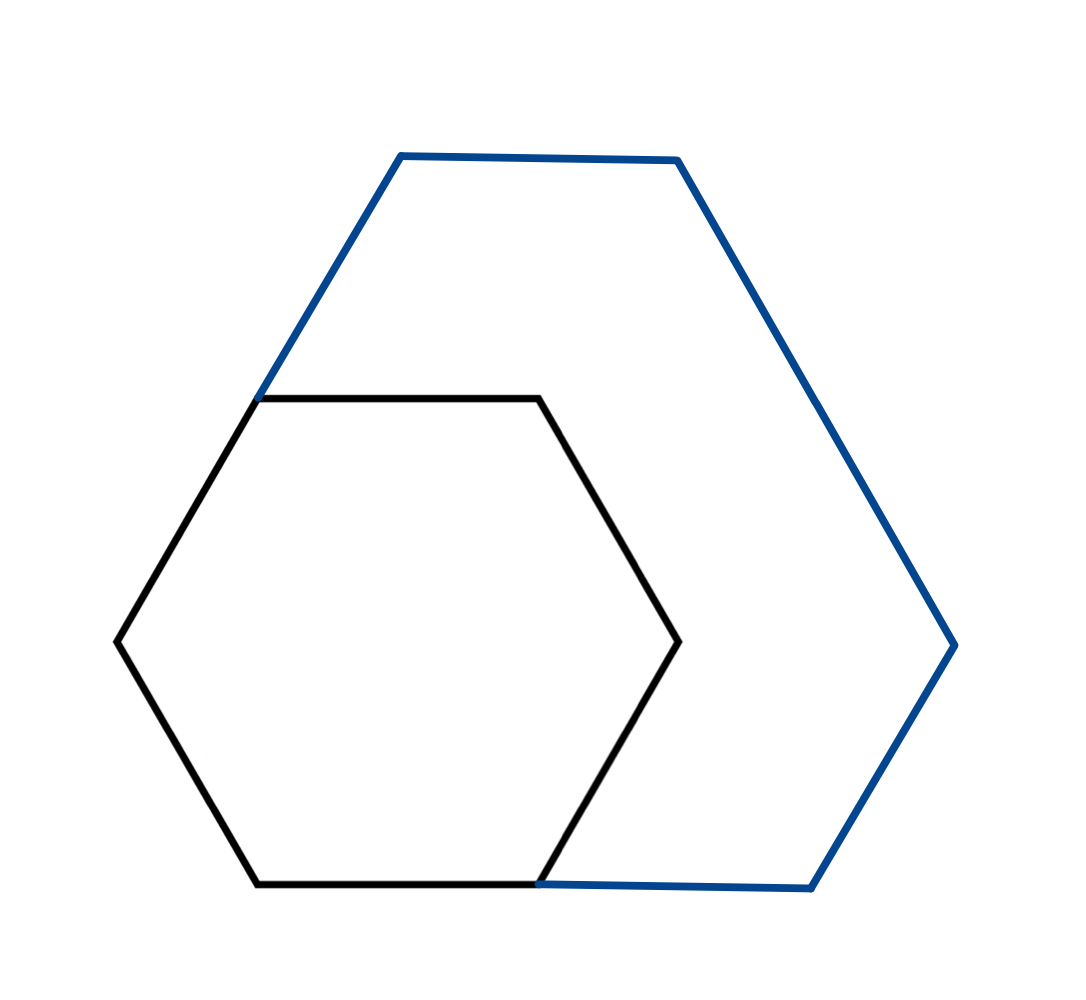
\includegraphics[scale=0.08]{images/P_C_3.png}
     \end{center}
\end{column}
\end{columns}    

\end{frame}



\begin{frame}{Reformulation of the theorem}
    \begin{corollary}
The volume of the generalized permutahedron $P_y^n(\{y_I\})$ is given by 
$$\text{Vol}\left( P_y^n(\{y_I\}) \right) = \frac{1}{(n-1)!} \sum_{(J_1, \dots, J_{n-1})} y_{J_1}, \dots, y_{J_{n-1}}$$
where the sum is given over ordered collections of subsets $J_1, \dots, J_{n-1} \in 2^{[n]}$ such that, for any distinct indices $i_1, \dots, i_k$ of the $J$'s, we have $|J_{i_1}\cup \ldots \cup J_{i_k}| \geq k+1$.
\end{corollary}
\end{frame}


\begin{frame}{Special case: Simplicial complex polytopes}
How can we understand the tuples of sets $(J_1,\ldots,J_{n-1})$ for a given simplicial complex in $n$ vertices?

\pause
\vspace{0.7cm}

\begin{definition}[C-tangram game]
Given a simplicial complex $C$, fix the 0-skeleton of $C$. You have the simplices in $C$ as your pieces of the game. \pause A \textbf{winning set} is a collection of $n-1$ pieces such that
\pause
\begin{itemize}
    \item The number of vertices joined using any $k$-subset of the pieces is greater than k. 
    \pause
    \item If a piece has dimension $d$, it can be repeated at most $d$ times. 
\end{itemize}
\end{definition}

\end{frame}

\begin{frame}{C-tangram game: Motivation}
\pause
    \begin{figure}
        \centering
        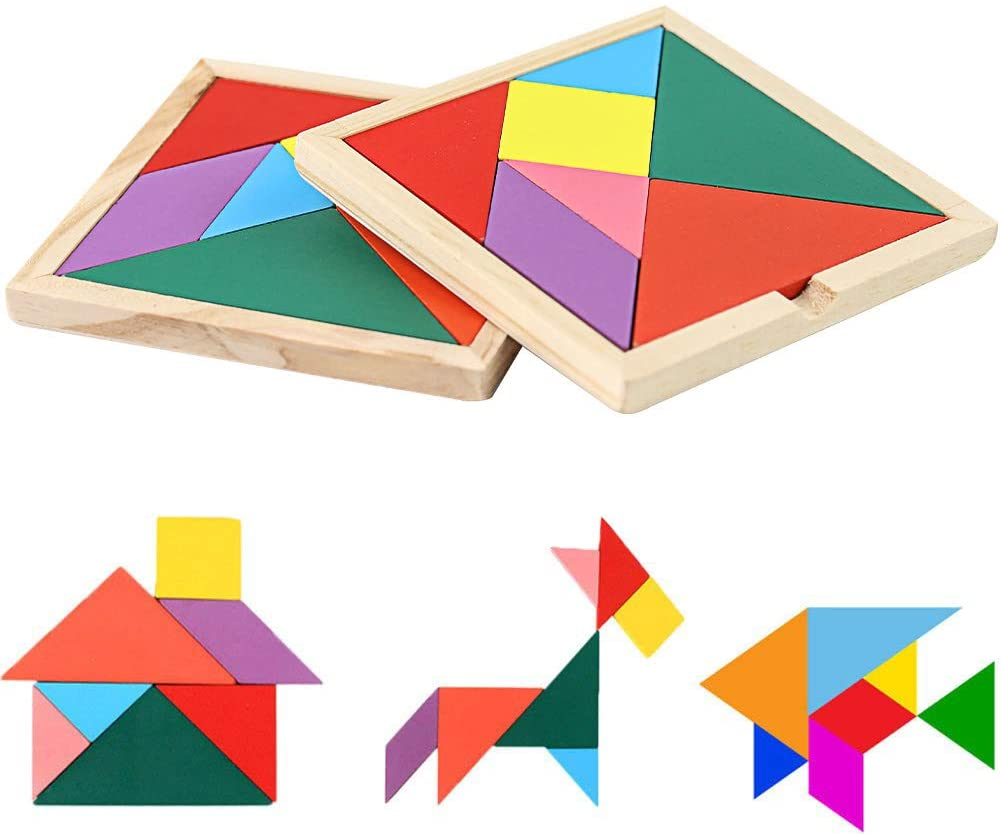
\includegraphics[scale=0.2]{images/tangram.jpg}
        \label{fig:tangram}
    \end{figure}
\pause
\vspace{0.5cm}
\small \textit{\textcolor{red}{Question}: Is this subdivision of the square regular?}
\end{frame}

\begin{frame}{C-tangram game}

Each winning set ${W}$ contributes in the sum of the volume of $P_C$ by the number of permutations it allows. \pause Lets call this number the \textbf{multiplicity of the winning set} and denote it by $m({W})$. \pause Explicitly, if ${W}$ has $W_1,\ldots,W_m$ \textit{distinct} simplices, each repeated $i_j$ times, then $$m({W}) = {{n}\choose {i_1,\ldots,i_m}}.$$ \pause Then, $$\text{vol}(P_C) = \frac{1}{(n-1)!} \; {\sum}_{{W}} \; m({W})$$ where the sum runs over all winning sets ${W}$ of the $C$-Tangram game.

    
\end{frame}

\begin{frame}{C-tangram game}
\begin{columns}
\begin{column}{0.5\textwidth}
   \begin{figure}
        \centering
        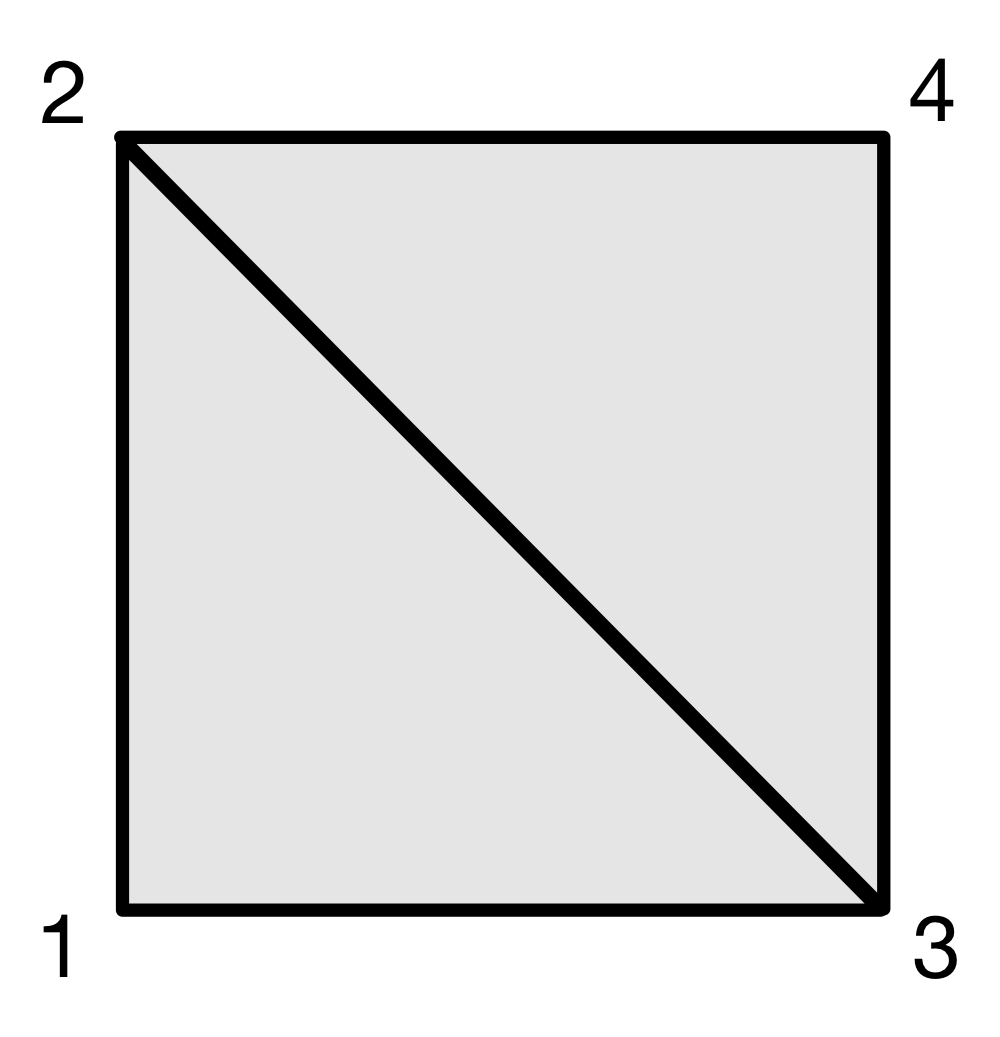
\includegraphics[scale=0.1]{images/SimpComplex.png}
    \end{figure}
\end{column}
\pause
\begin{column}{0.5\textwidth}  %%<--- here
    \begin{center}
     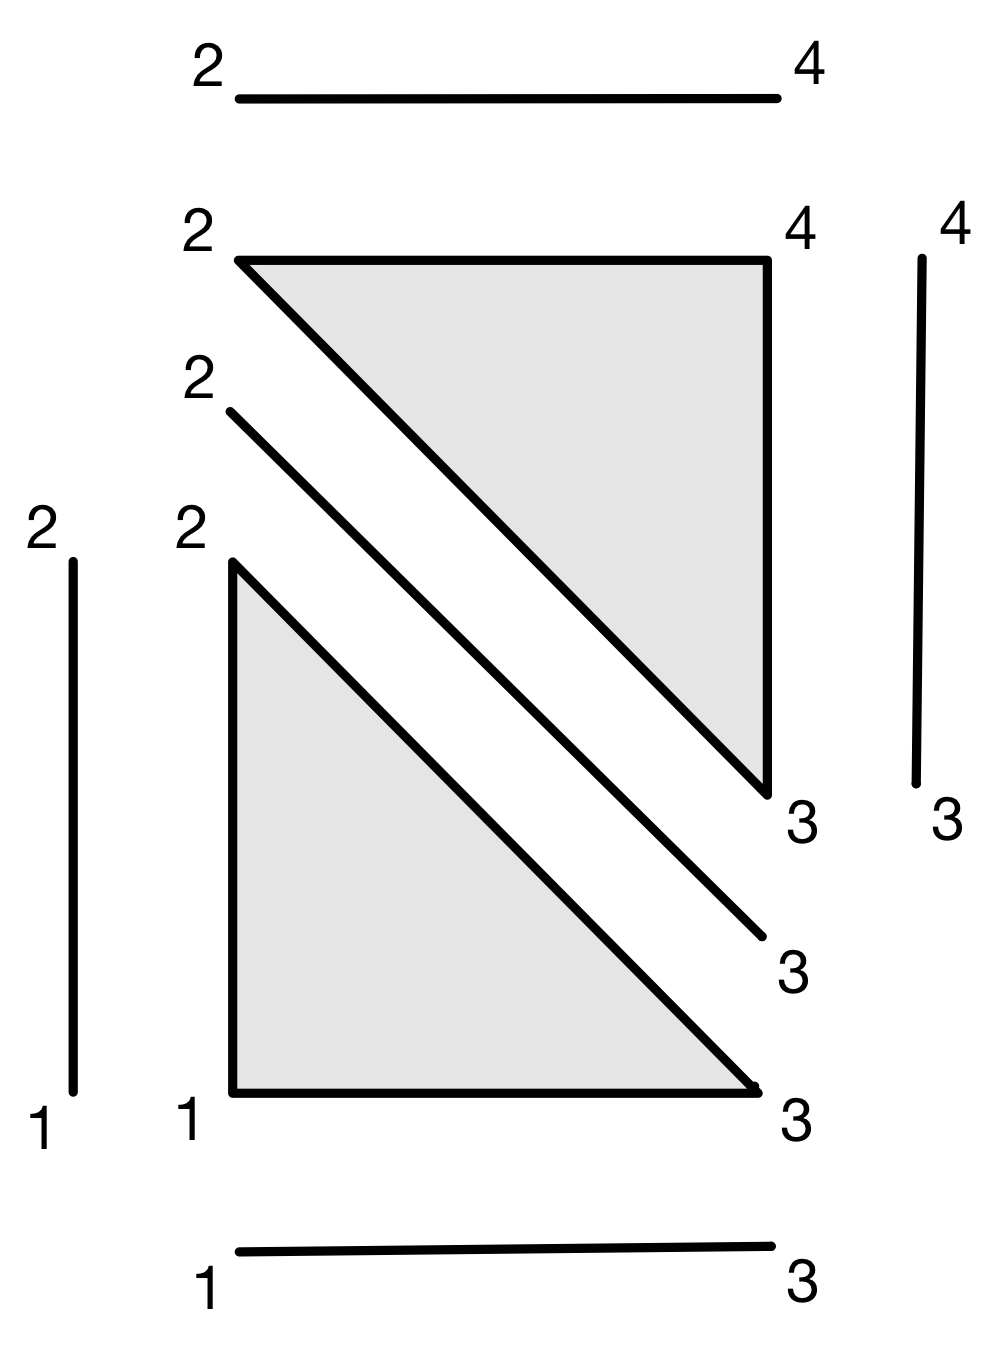
\includegraphics[scale=0.14]{images/Pieces.png}
     \end{center}
\end{column}
\end{columns}
\end{frame}

\begin{frame}{C-tangram game}
    \begin{figure}
        \centering
        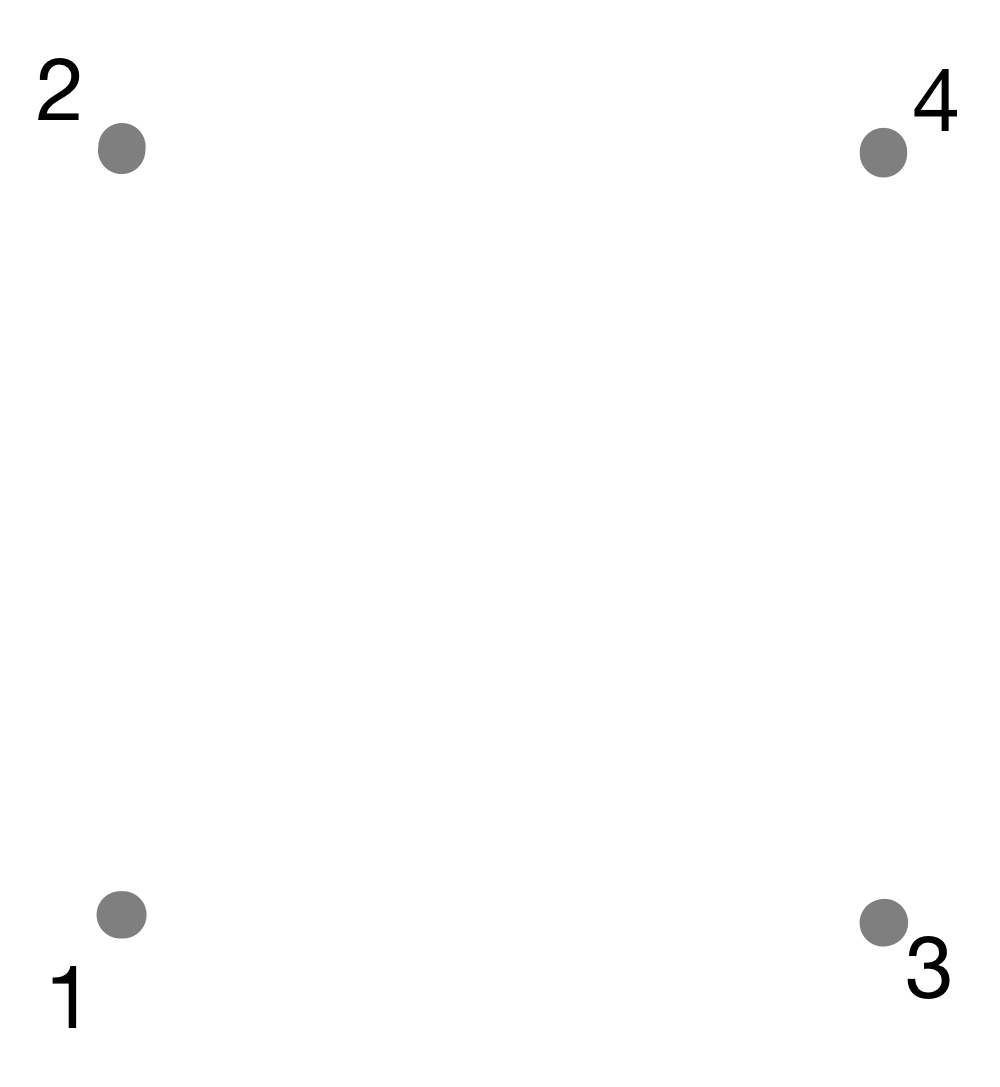
\includegraphics[scale=0.16]{images/0-skeleton.png}
    \end{figure}
\end{frame}

\begin{frame}{C-tangram game}
    \begin{figure}
        \centering
        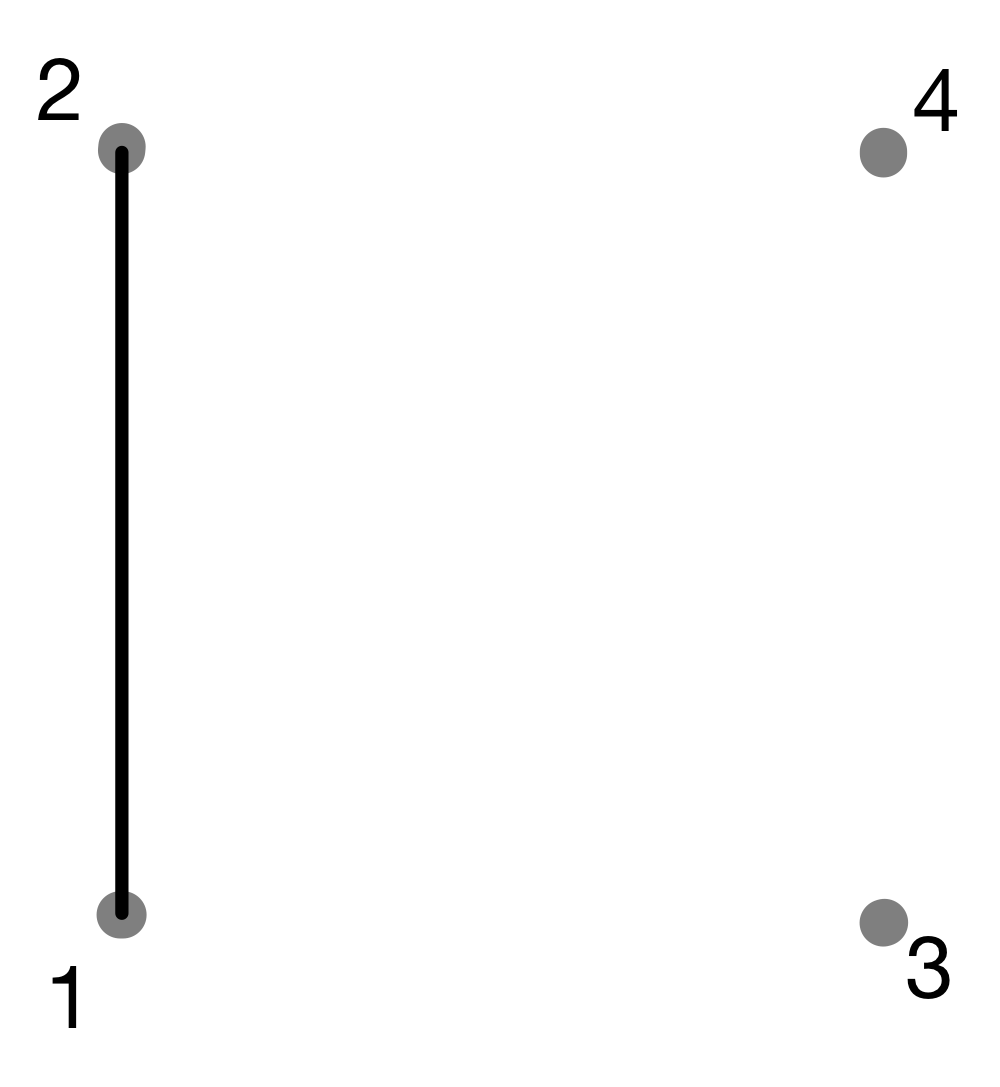
\includegraphics[scale=0.16]{images/Step1.png}
    \end{figure}
\end{frame}

\begin{frame}{C-tangram game}
    \begin{figure}
        \centering
        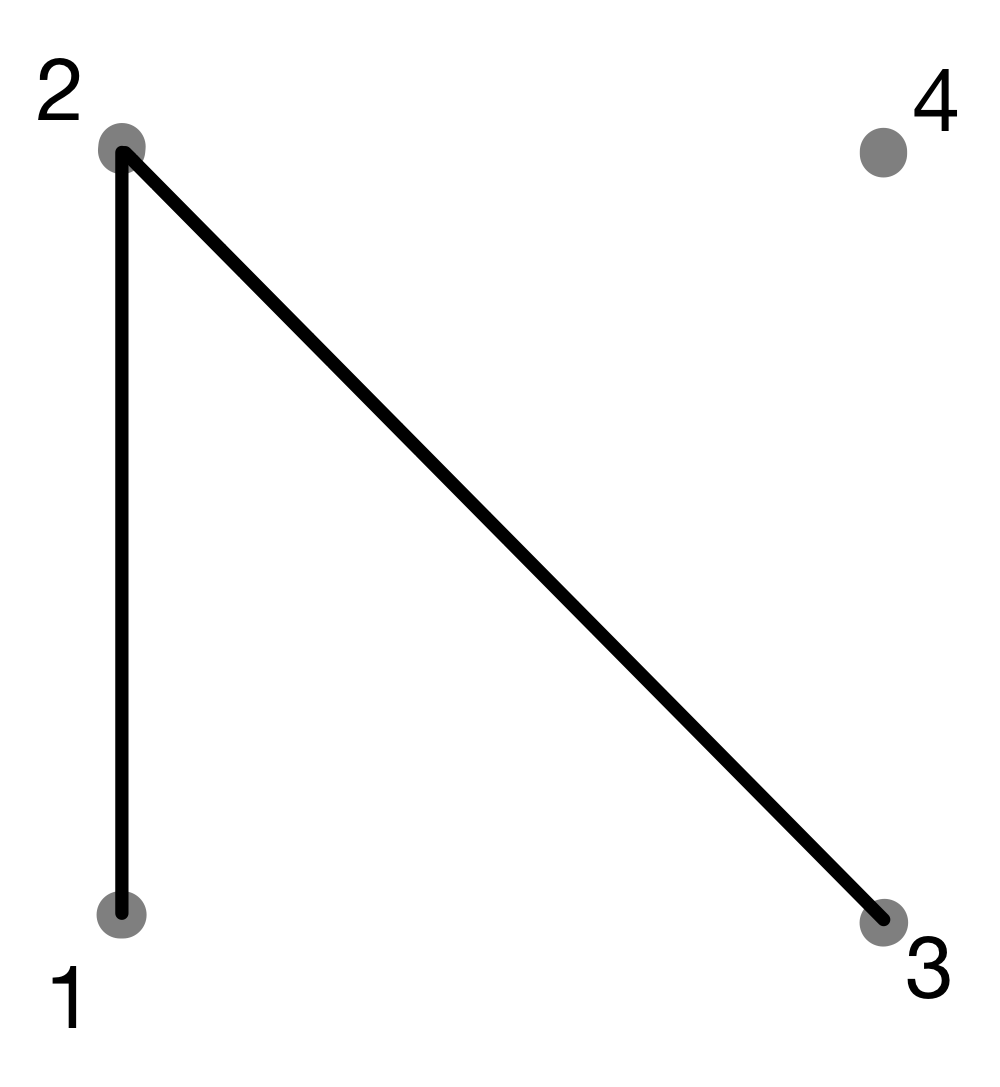
\includegraphics[scale=0.16]{images/Step2.png}
    \end{figure}
\end{frame}

\begin{frame}{C-tangram game}
    \begin{figure}
        \centering
        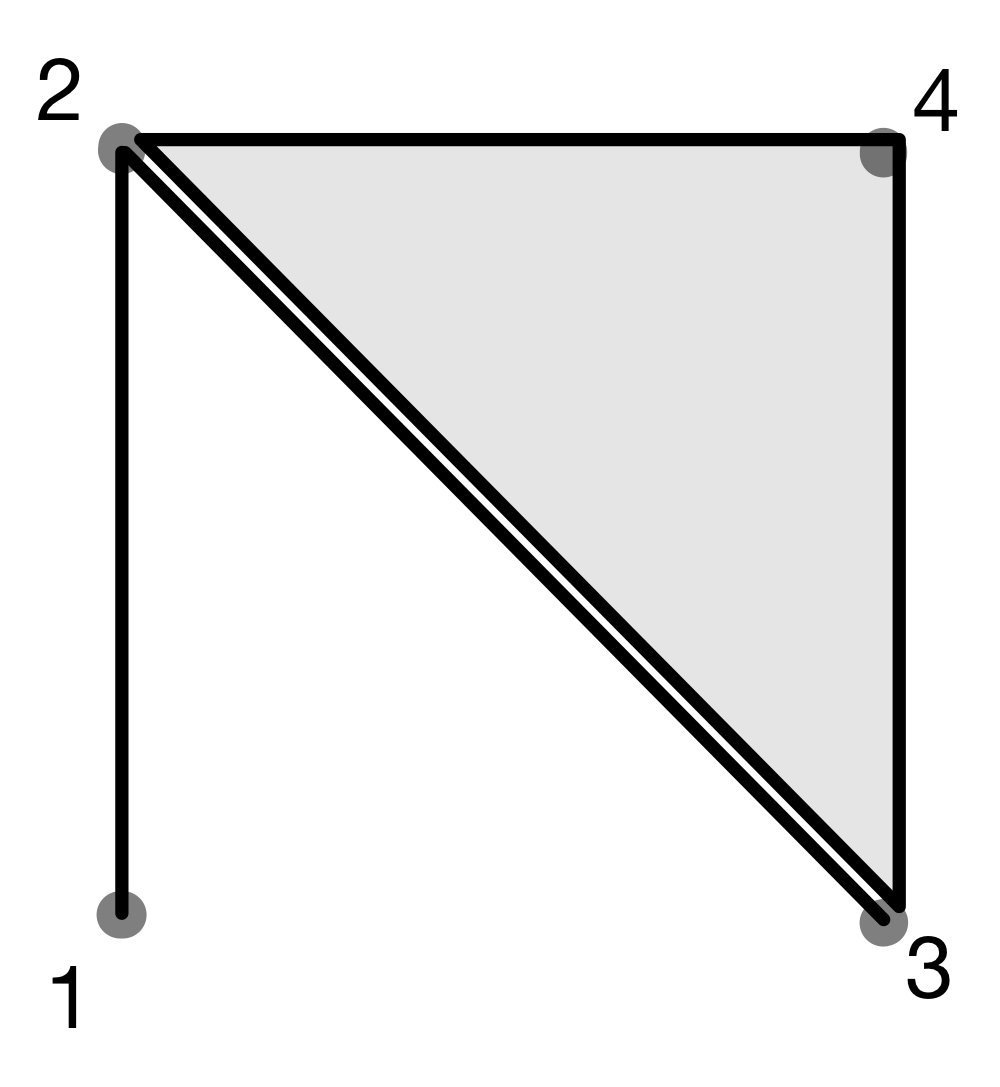
\includegraphics[scale=0.16]{images/Step3.png}
    \end{figure}
\end{frame}

\begin{frame}{C-tangram game}
However, this type of winning sets occur...
    \begin{figure}
        \centering
        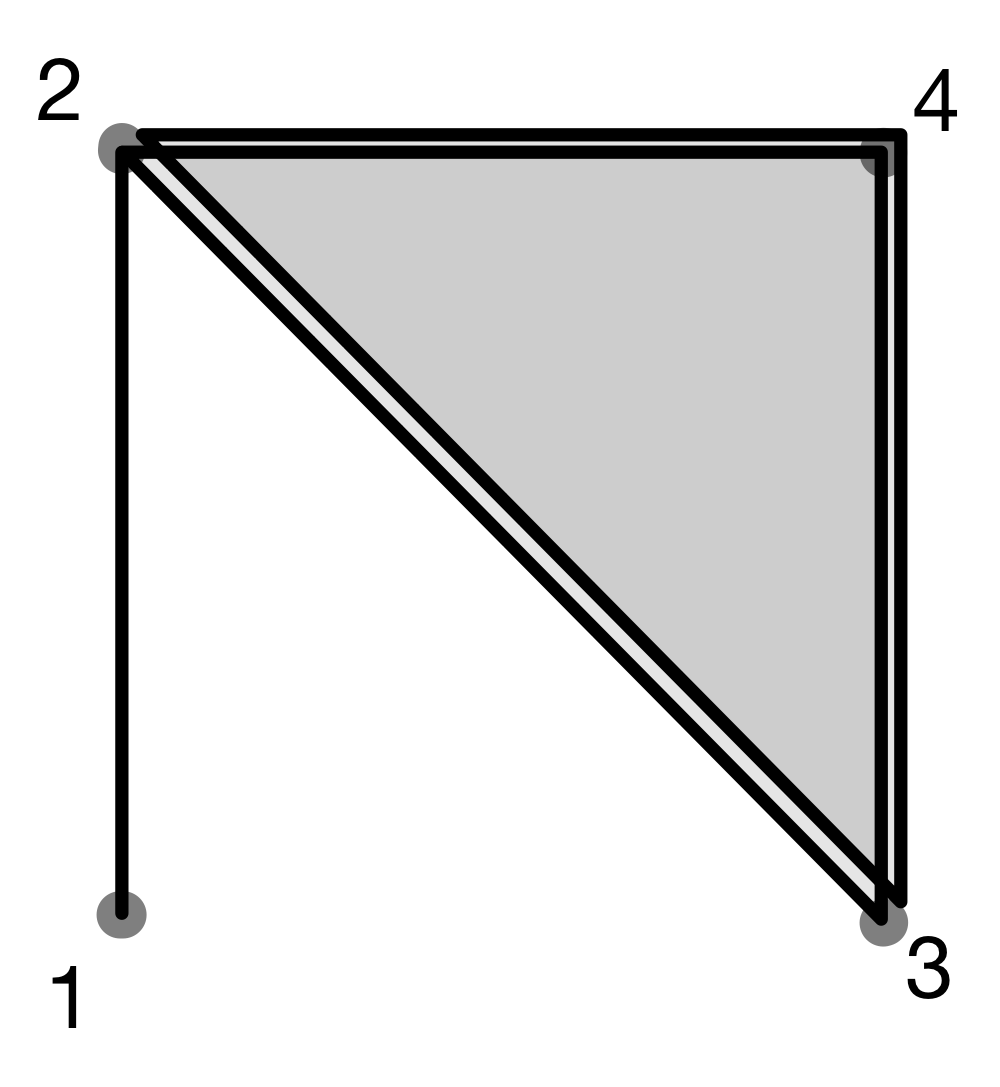
\includegraphics[scale=0.15]{images/Another.png}
    \end{figure}
\end{frame}

\begin{frame}{Winning sets}
How to obtain all winning sets for a particular simplicial complex?
\pause
\textbf{Using spanning trees!}
\pause
\begin{columns}
\begin{column}{0.45\textwidth}
   \begin{figure}
        \centering
        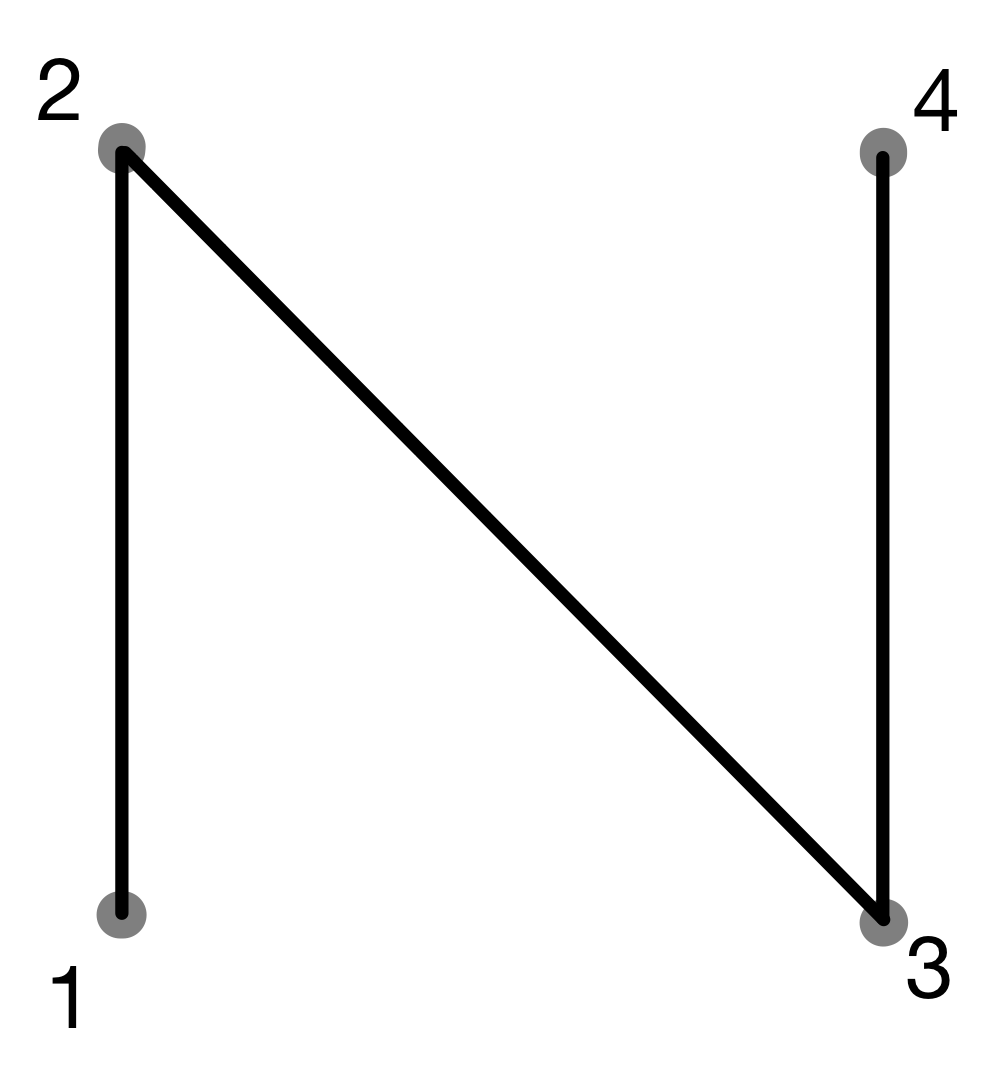
\includegraphics[scale=0.08]{images/SpanningTree.png}
    \end{figure}
\end{column}
\pause\begin{column}{0.1\textwidth}
$$\Large \xrightarrow{34\,\mapsto 234}$$
\end{column}
\pause
\begin{column}{0.45\textwidth} 
    \begin{center}
     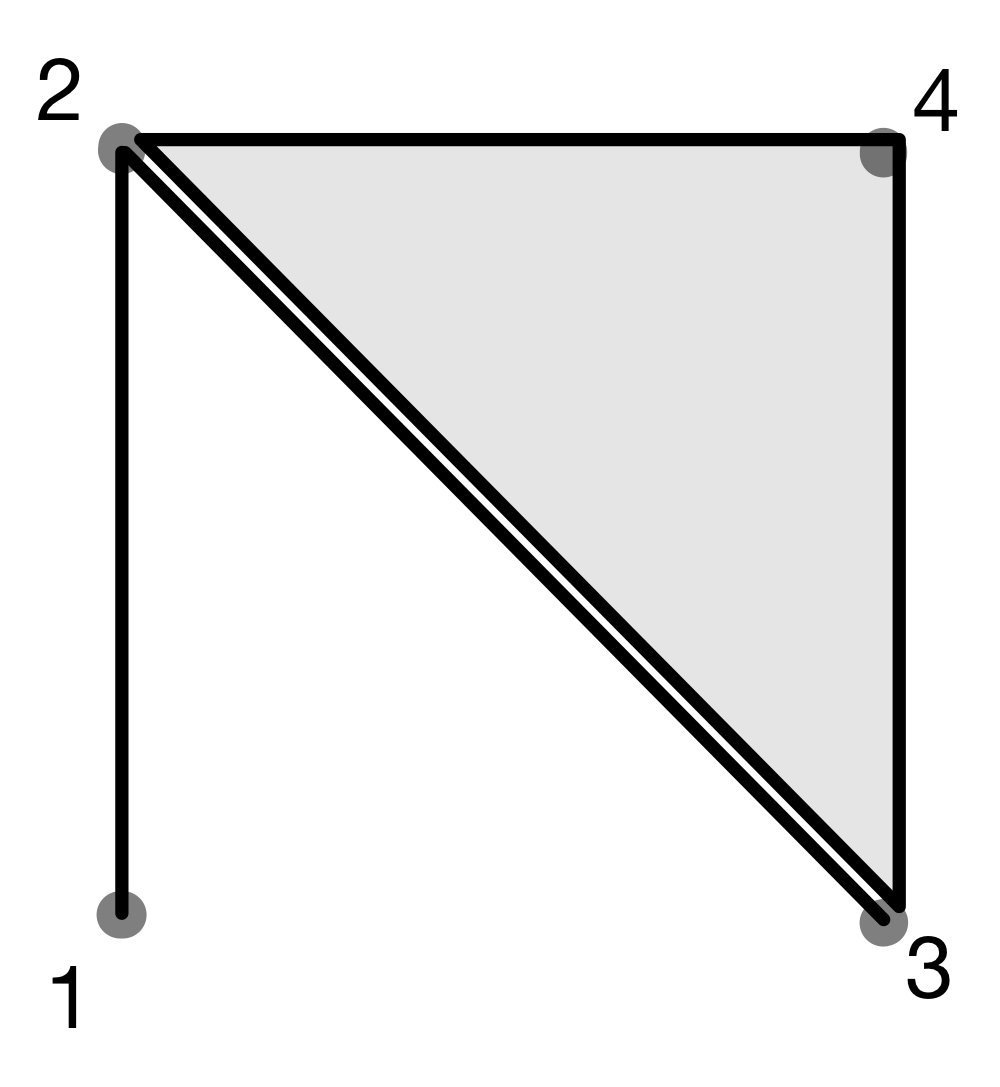
\includegraphics[scale=0.08]{images/Step3.png}
     \end{center}
\end{column}
\end{columns}
\vspace{0.5cm}
\pause

But this is not injective... 
\end{frame}

\begin{frame}{Winning sets algorithm}

\begin{enumerate}
    \pause
    \item[0.] List the complex\pause: $C = \{ 12,13,23,24,34,123,234 \}$
    \pause
    \item Search all spanning trees of the 1-skeleton. 
    \pause
    \item For each tree, order its edges and create the matrix $M_{ij} = 1$ iff $\tau_i \in S_j$ \pause : $\tau = \{12,23,24\}$ \pause and $$ M = \left( \begin{matrix} 1 & 0 & 0 & 0 & 0 & 1 & 0 \\ 0 & 0 & 1 & 0 & 0 & 1 & 1 \\ 0 & 0 & 0 & 1 & 0 & 0 & 1 \end{matrix} \right) $$
    \pause
    \item Pick a 1 from each row in all possible ways. 
    \pause
    \item Remove repetitions. 
\end{enumerate}
    
\end{frame}

\begin{frame}{Quick summary}
\pause
\begin{itemize}
    \item For a simplicial complex $C$, $P_C$ is a generalized permutahedron. 
    \item From Postnikov's theorem, the volume of $P_C$ can be computed.
    \item Using $C$-tangram winning sets with multiplicities, the volume of $P_C$ can be computed.
    \item Winning sets can be obtained from spanning trees of the 1-skeleton of the complex by doing swaps.
    
\end{itemize}
    
\end{frame}

\begin{frame}{Questions}
\begin{itemize}
    \item The winning sets give information of a subdivision of $P_C$ arising from the zonotopal subdivision of the graphical zonotope of $C^{(1)}$.
    \item Can the efficiency of the algorithm be improved?
    \item Is there a family of simplicial complexes with a \textit{nice} formula for its volume?
    \item As generalized permutahedra form a Hopf algebra, is there an algebraic way of computing the volume?
\end{itemize}    
\end{frame}

\begin{frame}{Questions}
    \begin{itemize}
    \item The winning sets give information of a subdivision of $P_C$ arising from the zonotopal subdivision of the graphical zonotope of $C^{(1)}$.
    
    \pause
    \textcolor{red}{Example:} For the complete complex in 3 vertices:
    \begin{figure}
        \centering
        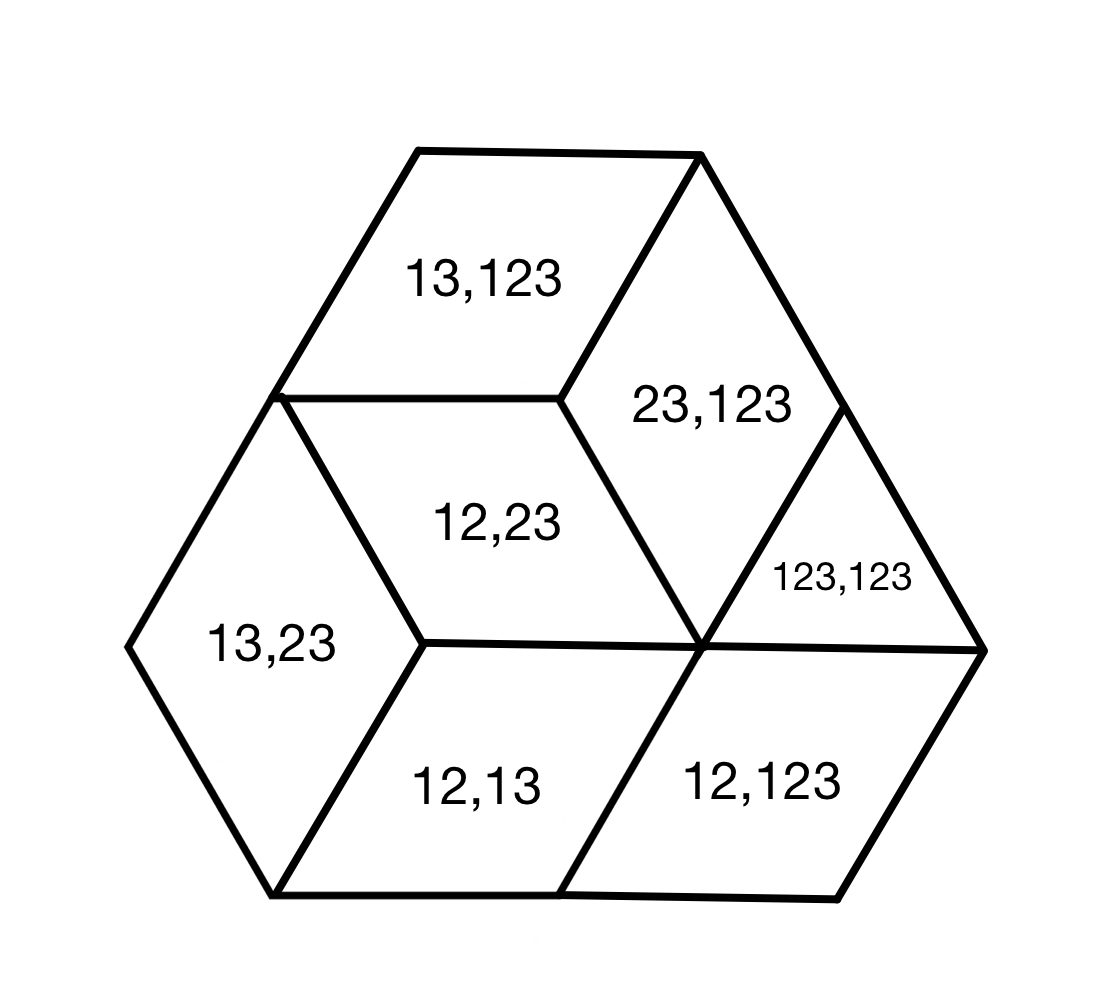
\includegraphics[scale=0.15]{images/P_C_3-subdivision-marked.png}
    \end{figure}
    \end{itemize}
\end{frame}

\begin{frame}
    \begin{center}
        \Huge Thanks! \\
    
        \Huge ¡Gracias!
    \end{center}
    
\end{frame}

\begin{frame}{References}
    \nocite{*}
    \printbibliography
\end{frame}

\end{document}
